\subsection{研究背景}
大语言模型（Large Language Model, LLM）已从离线批量生成，转变为支撑对话、检索增强、代码补全与智能体等交互式服务的核心组件\cite{yu2022orca,kwon2023vllm}。这类服务对单次响应时延高度敏感：一次请求首先并行处理输入序列以产生首个 token（prefill），随后依据已缓存的 Key-Value Cache（KV Cache）逐 token 解码（decode）\cite{zhong2024distserve,agrawal2024sarathiServe}。与追求峰值吞吐的训练范式不同，交互式推理的大量计算落在单次计算量很小的区间——小 batch 的 decode、短增量的 prefill，以及智能体在工具调用前后需要快速返回的阶段\cite{luo2026agentix}。在这一阶段暴露出两个重要问题：首先，低 batch 推理处于与训练截然不同的约束下，其主要瓶颈并非算力，而是全局内存与片上内存之间频繁搬运带来的内存带宽成本\cite{dao2022flashattention,nrusimha2025flashformer}；其次，为每层 Transformer 启动多个独立内核所引入的内核启动开销，也可能上升为瓶颈\cite{nrusimha2025flashformer,vellaisamy2026taxbreak}。尤其在低时延约束的场景中，这些近乎固定的开销无法被充分的计算所摊薄，会在端到端时延中占据不可忽视的比例。而解决这两类问题的主要做法，是算子融合与启动开销的消除\cite{chen2018tvm,niu2021dnnfusion,shi2023welder,nvidia2026cudaGraphs}。

具体而言，一层 Transformer 推理通常被拆成归一化、线性变换、位置编码、Attention、激活函数和残差连接等多个 GPU 计算阶段；各阶段若以独立 kernel 串行执行，中间张量便需反复写回 HBM，并在阶段边界支付启动与同步代价。FlashAttention 从 Attention 内部重排数据流以降低 HBM 访问；TVM、DNNFusion、Welder 则分别在计算图、融合计划与 tile-graph 层面压缩算子边界、扩大片上复用。这些工作共同表明：低时延推理的性能，取决于算子内部实现与算子之间执行边界的协同设计\cite{dao2022flashattention,chen2018tvm,niu2021dnnfusion,shi2023welder}。

近期研究进一步将融合范围从局部算子扩展到 Transformer 层乃至完整解码主体。FlashFormer 这类 whole-model kernel 面向低 batch 推理，把整模型前向融合为单个 kernel\cite{nrusimha2025flashformer}；Hazy Research 以设备端指令解释器与 counter 同步，把 Llama 前向收进单一 megakernel，消除 kernel 边界带来的流水气泡\cite{hazy2025nobubbles,hazyMegakernels2025}；MPK 进一步把张量程序降低为 SM 级任务图，并在 persistent megakernel 中去中心化调度\cite{cheng2025mpk}；DeepGEMM 的 MegaMoE 则在 SM90 上把 dispatch、专家侧 GEMM、SwiGLU 与 combine 等阶段组织进同一 cooperative kernel\cite{deepgemm2026,deepgemmPr360}；Event Tensor 把跨任务依赖提升为可编译的事件张量抽象，以支持动态 shape 与数据依赖调度\cite{eventTensor2026}。这类执行方式统称为 Megakernel：CPU 只发起一次或少量物理 CUDA launch，一组 persistent 或 cooperative workers 在 GPU 内部连续执行多个算子任务，并通过 queue、event、counter 或 grid-wide synchronization 表达跨算子依赖。

图~\ref{fig:megakernel-principle} 对比同一条 $A\!\rightarrow\!B\!\rightarrow\!C$ 算子链的三种执行映射：多 kernel、传统编译期融合，以及 persistent Megakernel。前两者仍依赖物理 grid 边界排序阶段；Megakernel 则一次 launch，把任务投放与依赖判断下沉到设备端，从而在依赖允许时形成跨任务流水。

\usetikzlibrary{arrows.meta}
\begin{figure}[htbp]
  \centering
  % shift={(...)} 使用坐标系单位；勿用 xshift=..cm，否则面板间距会被放大约 1/x 倍。
  \makebox[\textwidth][c]{%
  \resizebox{1.12\textwidth}{!}{%
  \begin{tikzpicture}[
      x=0.82cm,
      y=0.60cm,
      font=\scriptsize,
      panel/.style={
        draw=black!28,
        rounded corners=1.5pt,
        line width=0.35pt
      },
      lane/.style={
        draw=black!14,
        line width=0.3pt
      },
      lanelabel/.style={
        anchor=east,
        font=\fontsize{5}{6}\selectfont,
        text=black!72,
        align=right
      },
      ctrl/.style={
        draw=violet!55!black,
        fill=violet!10,
        rounded corners=1pt,
        line width=0.45pt
      },
      taskA/.style={
        draw=blue!65!black,
        fill=blue!14,
        rounded corners=0.8pt,
        line width=0.45pt
      },
      taskB/.style={
        draw=orange!80!black,
        fill=orange!18,
        rounded corners=0.8pt,
        line width=0.45pt
      },
      taskC/.style={
        draw=teal!65!black,
        fill=teal!15,
        rounded corners=0.8pt,
        line width=0.45pt
      },
      launchbox/.style={
        draw=black!70,
        fill=black!7,
        rounded corners=0.7pt,
        line width=0.4pt
      },
      boundary/.style={
        draw=black!55,
        densely dashed,
        line width=0.45pt
      },
      dispatch/.style={
        -{Latex[length=1.3mm]},
        draw=violet!70!black,
        densely dotted,
        line width=0.5pt
      },
      dep/.style={
        -{Latex[length=1.3mm]},
        draw=blue!70!black,
        line width=0.55pt
      },
      spill/.style={
        {Latex[length=1.2mm]}-{Latex[length=1.2mm]},
        draw=red!65!black,
        line width=0.55pt
      },
      wait/.style={
        draw=black!30,
        fill=black!5,
        densely dashed,
        rounded corners=0.7pt,
        line width=0.35pt
      },
      memory/.style={
        draw=black!45,
        fill=black!6,
        rounded corners=0.8pt,
        line width=0.4pt
      }
    ]

    % ======================================================================
    % (a) Separate physical kernels
    % ======================================================================
    \begin{scope}[shift={(0,0)}]
      \draw[panel] (0.05,0.10) rectangle (7.05,7.20);

      \node[font=\small\bfseries] at (3.60,6.82)
        {(a) 多 kernel};

      \foreach \yy in {5.90,5.05,4.05,3.35,2.65} {
        \draw[lane] (1.70,\yy) -- (6.85,\yy);
      }

      \node[lanelabel] at (1.58,5.90) {Host};
      \node[lanelabel] at (1.58,5.05) {Grid ctrl.};
      \node[lanelabel] at (1.58,4.05) {SM 0};
      \node[lanelabel] at (1.58,3.35) {SM 1};
      \node[lanelabel] at (1.58,2.65) {SM $n$};
      \node[lanelabel] at (1.58,1.55) {HBM};

      \draw[launchbox] (1.75,5.69) rectangle (2.22,6.11);
      \node[font=\tiny] at (1.985,5.90) {$L_A$};
      \draw[launchbox] (3.20,5.69) rectangle (3.67,6.11);
      \node[font=\tiny] at (3.435,5.90) {$L_B$};
      \draw[launchbox] (4.75,5.69) rectangle (5.22,6.11);
      \node[font=\tiny] at (4.985,5.90) {$L_C$};

      \draw[ctrl] (1.85,4.84) rectangle (3.05,5.26);
      \node[font=\tiny] at (2.45,5.05) {grid $A$};
      \draw[ctrl] (3.35,4.84) rectangle (4.60,5.26);
      \node[font=\tiny] at (3.975,5.05) {grid $B$};
      \draw[ctrl] (4.90,4.84) rectangle (6.40,5.26);
      \node[font=\tiny] at (5.65,5.05) {grid $C$};

      \foreach \yy in {4.05,3.35,2.65} {
        \draw[taskA] (1.85,\yy-0.21) rectangle (3.05,\yy+0.21);
        \node[font=\tiny] at (2.45,\yy) {$A$};
        \draw[taskB] (3.35,\yy-0.21) rectangle (4.60,\yy+0.21);
        \node[font=\tiny] at (3.975,\yy) {$B$};
        \draw[taskC] (4.90,\yy-0.21) rectangle (6.40,\yy+0.21);
        \node[font=\tiny] at (5.65,\yy) {$C$};
      }

      \draw[boundary] (3.20,2.35) -- (3.20,5.40);
      \draw[boundary] (4.75,2.35) -- (4.75,5.40);
      \node[font=\fontsize{4.5}{5}\selectfont,fill=white,inner sep=0.5pt,text=black!65]
        at (3.20,4.52) {grid 完成};

      \draw[memory] (1.70,1.33) rectangle (6.85,1.77);
      \node[font=\fontsize{5}{6}\selectfont,text=black!70] at (4.275,1.55)
        {输入 / 中间结果 / 输出};

      \draw[spill] (3.20,1.79) -- node[right,font=\tiny] {$I_A$} (3.20,2.42);
      \draw[spill] (4.75,1.79) -- node[right,font=\tiny] {$I_B$} (4.75,2.42);

      \draw[-{Latex[length=1.5mm]},black!65]
        (1.70,0.82) -- (6.80,0.82)
        node[above left,inner sep=1pt,font=\tiny] {time};
      \node[font=\fontsize{5}{6}\selectfont\bfseries,text=black!72] at (4.275,0.38)
        {3 launches $\cdot$ 2 次全局 grid 边界};
    \end{scope}

    % ======================================================================
    % (b) Conventional compile-time operator fusion
    % ======================================================================
    \begin{scope}[shift={(7.18,0)}]
      \draw[panel] (0.05,0.10) rectangle (7.05,7.20);

      \node[font=\small\bfseries] at (3.60,6.82)
        {(b) 传统算子融合};

      \foreach \yy in {5.90,5.05,4.05,3.35,2.65} {
        \draw[lane] (1.70,\yy) -- (6.85,\yy);
      }

      \node[lanelabel] at (1.58,5.90) {Host};
      \node[lanelabel] at (1.58,5.05) {Grid ctrl.};
      \node[lanelabel] at (1.58,4.05) {SM 0};
      \node[lanelabel] at (1.58,3.35) {SM 1};
      \node[lanelabel] at (1.58,2.65) {SM $n$};
      \node[lanelabel] at (1.58,1.55) {HBM};

      \draw[launchbox] (1.75,5.69) rectangle (2.65,6.11);
      \node[font=\tiny] at (2.20,5.90) {$L_{A+B}$};
      \draw[launchbox] (4.65,5.69) rectangle (5.12,6.11);
      \node[font=\tiny] at (4.885,5.90) {$L_C$};

      \draw[ctrl] (1.85,4.84) rectangle (4.45,5.26);
      \node[font=\tiny] at (3.15,5.05) {grid $F_{A+B}$};
      \draw[ctrl] (4.80,4.84) rectangle (6.40,5.26);
      \node[font=\tiny] at (5.60,5.05) {grid $C$};

      \foreach \yy in {4.05,3.35,2.65} {
        \draw[taskA] (1.85,\yy-0.21) rectangle (2.85,\yy+0.21);
        \node[font=\tiny] at (2.35,\yy) {$A$};
        \draw[taskB] (2.85,\yy-0.21) rectangle (4.45,\yy+0.21);
        \node[font=\tiny] at (3.65,\yy) {$B$};
        \draw[taskC] (4.80,\yy-0.21) rectangle (6.40,\yy+0.21);
        \node[font=\tiny] at (5.60,\yy) {$C$};
      }

      \draw[boundary] (4.625,2.35) -- (4.625,5.40);

      \draw[memory] (1.70,1.33) rectangle (6.85,1.77);
      \node[font=\fontsize{5}{6}\selectfont,text=black!70] at (4.275,1.55)
        {输入 / 融合输出 / 最终输出};

      \draw[spill] (4.625,1.79)
        -- node[right,font=\tiny] {$I_{A+B}$} (4.625,2.42);

      \draw[-{Latex[length=1.5mm]},black!65]
        (1.70,0.82) -- (6.80,0.82)
        node[above left,inner sep=1pt,font=\tiny] {time};
      \node[font=\fontsize{5}{6}\selectfont\bfseries,text=black!72] at (4.275,0.38)
        {2 launches $\cdot$ grid 内静态融合};
    \end{scope}

    % ======================================================================
    % (c) Persistent megakernel with an on-device scheduler
    % ======================================================================
    \begin{scope}[shift={(14.36,0)}]
      \draw[panel] (0.05,0.10) rectangle (7.05,7.20);

      \node[font=\small\bfseries] at (3.60,6.82)
        {(c) Persistent Megakernel};

      \foreach \yy in {5.90,5.05,4.05,3.35,2.65} {
        \draw[lane] (1.70,\yy) -- (6.85,\yy);
      }

      \node[lanelabel] at (1.58,5.90) {Host};
      \node[lanelabel] at (1.58,5.05) {Sched. SM};
      \node[lanelabel] at (1.58,4.05) {SM 0};
      \node[lanelabel] at (1.58,3.35) {SM 1};
      \node[lanelabel] at (1.58,2.65) {SM $n$};
      \node[lanelabel] at (1.58,1.55) {HBM};

      \draw[launchbox] (1.75,5.69) rectangle (2.33,6.11);
      \node[font=\tiny] at (2.04,5.90) {$L_M$};

      \draw[
        draw=teal!55!black,
        densely dashed,
        rounded corners=1.2pt,
        line width=0.55pt
      ] (1.78,2.32) rectangle (6.45,5.34);

      \node[
        font=\fontsize{5}{6}\selectfont\bfseries,
        fill=white,
        inner sep=0.5pt,
        text=teal!55!black
      ] at (5.45,5.48) {persistent grid};

      \draw[ctrl] (1.90,4.83) rectangle (6.30,5.27);
      \node[font=\fontsize{5}{6}\selectfont] at (4.10,5.05)
        {ready queue / events / counters};

      % Worker SM 0
      \draw[taskA] (1.95,3.84) rectangle (2.68,4.26);
      \node[font=\tiny] at (2.315,4.05) {$A_0$};
      \draw[taskB] (2.83,3.84) rectangle (3.58,4.26);
      \node[font=\tiny] at (3.205,4.05) {$B_0$};
      \draw[wait] (3.65,3.84) rectangle (4.85,4.26);
      \node[font=\tiny,text=black!50] at (4.25,4.05) {wait};
      \draw[taskC] (4.92,3.84) rectangle (5.72,4.26);
      \node[font=\tiny] at (5.32,4.05) {$C_0$};

      % Worker SM 1
      \draw[taskA] (2.10,3.14) rectangle (2.85,3.56);
      \node[font=\tiny] at (2.475,3.35) {$A_1$};
      \draw[taskB] (3.00,3.14) rectangle (3.75,3.56);
      \node[font=\tiny] at (3.375,3.35) {$B_1$};
      \draw[wait] (3.82,3.14) rectangle (4.98,3.56);
      \node[font=\tiny,text=black!50] at (4.40,3.35) {wait};
      \draw[taskC] (5.05,3.14) rectangle (5.85,3.56);
      \node[font=\tiny] at (5.45,3.35) {$C_1$};

      % Worker SM n
      \draw[taskA] (2.30,2.44) rectangle (3.10,2.86);
      \node[font=\tiny] at (2.70,2.65) {$A_n$};
      \draw[taskB] (3.25,2.44) rectangle (4.30,2.86);
      \node[font=\tiny] at (3.775,2.65) {$B_n$};
      \draw[wait] (4.37,2.44) rectangle (5.10,2.86);
      \node[font=\tiny,text=black!50] at (4.735,2.65) {wait};
      \draw[taskC] (5.17,2.44) rectangle (6.00,2.86);
      \node[font=\tiny] at (5.585,2.65) {$C_n$};

      \draw[dep] (2.68,4.31) -- (2.83,4.31);
      \node[
        font=\fontsize{4.5}{5}\selectfont,
        anchor=south,
        text=blue!70!black
      ] at (2.75,4.36) {tile ready};

      \draw[dispatch] (2.85,4.82) -- (2.85,4.30);
      \draw[dispatch] (5.15,4.82) -- (5.15,3.60);

      \draw[
        draw=red!65!black,
        densely dashed,
        line width=0.55pt
      ] (4.70,2.32) -- (4.70,4.70);
      \node[
        font=\fontsize{4.5}{5}\selectfont,
        anchor=south east,
        fill=white,
        inner sep=0.5pt,
        text=red!65!black
      ] at (4.62,4.36) {all ready};

      \draw[memory] (1.70,1.33) rectangle (6.85,1.77);
      \node[font=\fontsize{5}{6}\selectfont,text=black!70] at (4.275,1.55)
        {模型状态 / KV / 输出};

      \draw[-{Latex[length=1.2mm]},draw=black!55]
        (2.20,1.78) -- (2.20,2.30);
      \draw[-{Latex[length=1.2mm]},draw=black!55]
        (6.05,2.30) -- (6.05,1.78);

      \draw[-{Latex[length=1.5mm]},black!65]
        (1.70,0.82) -- (6.80,0.82)
        node[above left,inner sep=1pt,font=\tiny] {time};
      \node[font=\fontsize{5}{6}\selectfont\bfseries,text=black!72] at (4.275,0.38)
        {1 launch $\cdot$ 设备端任务依赖};
    \end{scope}
  \end{tikzpicture}%
  }}%
  \caption{同一条 $A\!\rightarrow\!B\!\rightarrow\!C$ 算子链的三种执行映射。
  (a)~多 kernel 以物理 grid completion 排序阶段，并在边界处物化中间结果；
  (b)~传统融合消去 $A$--$B$ 物理边界，但 worker 仍执行静态融合程序，且 $C$ 前仍保留物理边界；
  (c)~persistent Megakernel 仅 launch 一次，由设备端调度维护 queue/event/counter，worker 拉取 tile 任务：
  tile-ready 允许 $B_0$ 与 $A$ 尾部重叠，而 $C$ 前的 all-ready 则表现为内部 readiness gate。
  Megakernel 中间结果是否落 HBM 取决于具体实现，图中不作约定。}
  \label{fig:megakernel-principle}
\end{figure}


然而，将多个算子放入同一个 Megakernel，并不会消除算子之间的数据依赖。原先由物理 kernel 边界隐式保证的算子间的同步关系，在融合之后仍须在设备端显式维护。以 Llama 解码阶段的计算图为例。在从（QKV/RoPE）到部分注意力（PartialAttention）的计算图连边上，注意力计算只需等待对应注意力头的QKV就绪，即可开始读取该注意力头的KV cache；因此，部分注意力头可以与尚未完成的其他注意力头的前驱计算重叠执行。相比之下，在从部分注意力到输出投影与残差连接（O-Proj/Residual）的计算图连边上，每一个输出投影都依赖完整的注意力输出张量；因此，只有全部 query head 对应的注意力结果都已产生后，后继的主体计算才能开始。这两种不同依赖形态决定了相邻算子边应映射到何种物理执行方式。对于前者，将生产者与消费者保留在同一 grid 内，并通过设备端事件同步，通常能够获得有效的计算重叠。然而对于后者，过早地在同一 grid 内启动消费者往往无法形成有用重叠，却仍需承担设备端等待与跨阶段交接的开销；此时，用物理 grid 完成语义分隔前后阶段，反而可能更有利。因此，减少一次 kernel launch 与减少一次同一 grid 内的软件同步，构成方向相反的两项开销。

在这类 Megakernel 中，算子阶段还会被进一步划分成可并行调度的 task：PartialAttention 按注意力头分组，输出投影按输出行块划分。以 \texttt{PartialAttention}$\rightarrow$\texttt{O\_ProjResidual} 为例，8 个 PartialAttention task 共同产生 32 个 query head 的结果，128 个输出投影 task 却都要等这 32 个结果全部就绪后才能开始依赖计算。然而在执行时各 SM {O\_ProjResidual} task 会在全量就绪之前就被调度并进入等待。从依赖分析的角度来看，这种提前调度也无法带来注意力计算的有效重叠，却引入了相比于一次物理grid的SM退出同步再调度更大的开销，其区别如图~\ref{fig:hazy-boundary}所示。

\usetikzlibrary{arrows.meta,calc,positioning}
\begin{figure}[htbp]
  \centering
  \makebox[\textwidth][c]{%
  \resizebox{0.98\textwidth}{!}{%
  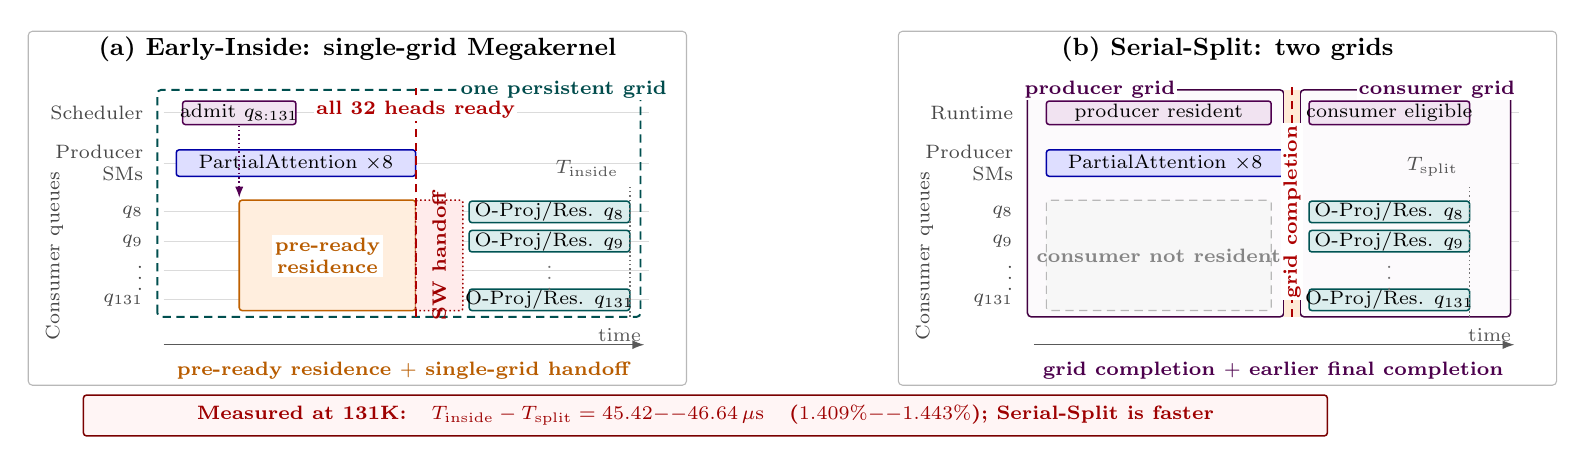
\begin{tikzpicture}[
      x=0.80cm,
      y=0.62cm,
      font=\sffamily\footnotesize,
      panel/.style={draw=black!28, rounded corners=1.5pt,
                    line width=0.4pt},
      lane/.style={draw=black!14, line width=0.3pt},
      lanelabel/.style={anchor=east, font=\scriptsize, text=black!72},
      producer/.style={draw=blue!65!black, fill=blue!13,
                       rounded corners=1pt, line width=0.55pt},
      consumer/.style={draw=teal!65!black, fill=teal!14,
                       rounded corners=1pt, line width=0.55pt},
      scheduler/.style={draw=violet!62!black, fill=violet!11,
                        rounded corners=1pt, line width=0.55pt},
      preready/.style={draw=orange!75!black, fill=orange!13,
                       rounded corners=1pt, line width=0.55pt},
      handoff/.style={draw=red!62!black, fill=red!8,
                      densely dotted, rounded corners=0.8pt,
                      line width=0.55pt},
      inactive/.style={draw=black!28, fill=black!3, densely dashed,
                       rounded corners=1pt, line width=0.4pt},
      persistgrid/.style={draw=teal!62!black, densely dashed,
                          rounded corners=1.4pt, line width=0.7pt},
      physicalgrid/.style={draw=violet!52!black, fill=violet!2,
                           rounded corners=1.4pt, line width=0.55pt},
      readyline/.style={draw=red!68!black, densely dashed,
                        line width=0.65pt},
      finishline/.style={draw=black!55, densely dotted,
                         line width=0.55pt},
      flow/.style={-{Latex[length=1.4mm]}, line width=0.55pt},
      result/.style={draw=red!48!black, fill=red!4,
                     rounded corners=1.2pt, line width=0.55pt}
    ]

    % ====================================================================
    % (a) Early-Inside
    % ====================================================================
    \begin{scope}[xshift=0cm]
      \draw[panel] (0,0) rectangle (10.45,7.25);
      \node[font=\small\bfseries] at (5.225,6.88)
        {(a) Early-Inside: single-grid Megakernel};

      % Shared resource lanes.
      \foreach \yy in {5.58,4.55,3.55,2.95,2.35,1.75} {
        \draw[lane] (2.15,\yy) -- (9.85,\yy);
      }
      \node[lanelabel] at (1.98,5.58) {Scheduler};
      \node[lanelabel,align=right] at (1.98,4.55) {Producer\\SMs};
      \node[font=\scriptsize,rotate=90,text=black!72] at (0.42,2.65)
        {Consumer queues};
      \node[lanelabel] at (1.98,3.55) {$q_8$};
      \node[lanelabel] at (1.98,2.95) {$q_9$};
      \node[lanelabel] at (1.98,2.35) {$\vdots$};
      \node[lanelabel] at (1.98,1.75) {$q_{131}$};

      % One persistent grid contains scheduler, producer, and consumers.
      \draw[persistgrid] (2.05,1.40) rectangle (9.72,6.05);
      \node[font=\scriptsize\bfseries,fill=white,inner sep=0.7pt,
            text=teal!60!black] at (8.50,6.05)
        {one persistent grid};

      % Device-side early admission.
      \draw[scheduler] (2.45,5.34) rectangle (4.25,5.82);
      \node[font=\scriptsize] at (3.35,5.58)
        {admit $q_{8{:}131}$};

      % Producer stage: eight tasks collectively make 32 query heads ready.
      \draw[producer] (2.35,4.28) rectangle (6.15,4.82);
      \node[font=\scriptsize] at (4.25,4.55)
        {PartialAttention $\times 8$};

      % Consumers are resident before the shared full-ready condition.
      \draw[preready] (3.35,1.53) rectangle (6.15,3.79);
      \node[font=\scriptsize\bfseries,align=center,
            fill=white,inner sep=1.1pt,text=orange!72!black]
        at (4.75,2.65) {pre-ready\\residence};

      % After full readiness, the single-grid path still performs a software
      % task handoff before the main consumer body can run.  The measured result
      % below, rather than an individual micro-event, establishes the gap.
      \draw[handoff] (6.15,1.53) rectangle (6.90,3.79);
      \node[font=\scriptsize\bfseries,rotate=90,text=red!62!black]
        at (6.525,2.65) {SW handoff};

      % Global all-ready condition shared by every consumer.
      \draw[readyline] (6.15,1.40) -- (6.15,6.08);
      \node[font=\scriptsize\bfseries,fill=white,inner sep=0.8pt,
            text=red!68!black] at (6.15,5.64)
        {all 32 heads ready};

      % Main consumer computation can start only after full readiness.
      \foreach \yy/\qq in {3.55/8,2.95/9,1.75/131} {
        \draw[consumer] (7.00,\yy-0.22) rectangle (9.55,\yy+0.22);
        \node[font=\scriptsize] at (8.275,\yy)
          {O-Proj/Res. $q_{\qq}$};
      }
      \node[font=\scriptsize,text=black!55] at (8.275,2.35) {$\vdots$};

      % End-to-end completion marker on the shared schematic time scale.
      \draw[finishline] (9.55,1.40) -- (9.55,4.06);
      \node[font=\scriptsize\bfseries,anchor=south east,
            text=black!68] at (9.52,4.08) {$T_{\mathrm{inside}}$};

      % Admission marker links the scheduler decision to consumer residence.
      \draw[flow,draw=violet!65!black,densely dotted]
        (3.35,5.32) -- (3.35,3.84);

      \draw[-{Latex[length=1.5mm]},black!65]
        (2.15,0.83) -- (9.78,0.83)
        node[above left,inner sep=1pt,font=\scriptsize] {time};
      \node[font=\scriptsize\bfseries,text=orange!72!black]
        at (5.95,0.30)
        {pre-ready residence $+$ single-grid handoff};
    \end{scope}

    % ====================================================================
    % (b) Serial-Split
    % ====================================================================
    \begin{scope}[xshift=11.05cm]
      \draw[panel] (0,0) rectangle (10.45,7.25);
      \node[font=\small\bfseries] at (5.225,6.88)
        {(b) Serial-Split: two grids};

      % Identical resource lanes and horizontal time scale.
      \foreach \yy in {5.58,4.55,3.55,2.95,2.35,1.75} {
        \draw[lane] (2.15,\yy) -- (9.85,\yy);
      }
      \node[lanelabel] at (1.98,5.58) {Runtime};
      \node[lanelabel,align=right] at (1.98,4.55) {Producer\\SMs};
      \node[font=\scriptsize,rotate=90,text=black!72] at (0.42,2.65)
        {Consumer queues};
      \node[lanelabel] at (1.98,3.55) {$q_8$};
      \node[lanelabel] at (1.98,2.95) {$q_9$};
      \node[lanelabel] at (1.98,2.35) {$\vdots$};
      \node[lanelabel] at (1.98,1.75) {$q_{131}$};

      % Two physical grids separated at the full-ready cut.
      \draw[physicalgrid] (2.05,1.40) rectangle (6.12,6.05);
      \draw[physicalgrid] (6.38,1.40) rectangle (9.72,6.05);
      \node[font=\scriptsize\bfseries,fill=white,inner sep=0.7pt,
            text=violet!58!black] at (3.20,6.05) {producer grid};
      \node[font=\scriptsize\bfseries,fill=white,inner sep=0.7pt,
            text=violet!58!black] at (8.55,6.05) {consumer grid};

      \draw[scheduler] (2.35,5.34) rectangle (5.92,5.82);
      \node[font=\scriptsize] at (4.135,5.58)
        {producer resident};

      \draw[producer] (2.35,4.28) rectangle (6.12,4.82);
      \node[font=\scriptsize] at (4.235,4.55)
        {PartialAttention $\times 8$};

      % Consumer queues are not admitted while the producer grid is active.
      \draw[inactive] (2.35,1.53) rectangle (5.92,3.79);
      \node[font=\scriptsize\bfseries,align=center,text=black!48]
        at (4.135,2.65) {consumer not resident};

      % Physical completion expresses the shared all-ready condition.
      \fill[orange!16] (6.12,1.40) rectangle (6.38,6.05);
      \draw[readyline] (6.25,1.40) -- (6.25,6.10);
      \node[font=\scriptsize\bfseries,rotate=90,fill=white,inner sep=0.8pt,
            text=red!68!black] at (6.25,3.55)
        {grid completion};

      \draw[scheduler] (6.52,5.34) rectangle (9.07,5.82);
      \node[font=\scriptsize] at (7.795,5.58)
        {consumer eligible};

      % The same consumer code begins only after the physical boundary.
      \foreach \yy/\qq in {3.55/8,2.95/9,1.75/131} {
        \draw[consumer] (6.52,\yy-0.22) rectangle (9.07,\yy+0.22);
        \node[font=\scriptsize] at (7.795,\yy)
          {O-Proj/Res. $q_{\qq}$};
      }
      \node[font=\scriptsize,text=black!55] at (7.795,2.35) {$\vdots$};

      \draw[finishline] (9.07,1.40) -- (9.07,4.06);
      \node[font=\scriptsize\bfseries,anchor=south east,
            text=black!68] at (9.04,4.08) {$T_{\mathrm{split}}$};

      \draw[-{Latex[length=1.5mm]},black!65]
        (2.15,0.83) -- (9.78,0.83)
        node[above left,inner sep=1pt,font=\scriptsize] {time};
      \node[font=\scriptsize\bfseries,text=violet!60!black]
        at (5.95,0.30)
        {grid completion $+$ earlier final completion};
    \end{scope}

    % The measured result makes the performance direction explicit.  The
    % timeline above is schematic; the numeric difference is the experiment.
    \node[result,minimum width=15.8cm,minimum height=0.52cm,
          font=\scriptsize\bfseries,text=red!62!black] at (10.75,-0.62)
      {Measured at 131K:\quad
       $T_{\mathrm{inside}}-T_{\mathrm{split}}
         =45.42\text{--}46.64\,\mu\mathrm{s}$\quad
       ($1.409\%\text{--}1.443\%$); Serial-Split is faster};

  \end{tikzpicture}%
  }}%
  \caption{Hazy \texttt{PartialAttention}$\rightarrow$\texttt{O\_ProjResidual} 的 SM--时间执行结构。Early-Inside 中，queues 8--131 在 32 个 query heads 全量就绪前进入 consumer 路径，形成 pre-ready residence interval；Serial-Split 由 producer grid completion 统一放行 consumer grid。两种方案保持 task code、queue mapping、task/noop slots 和 instruction bytes 一致。橙色区间对应后续 admission-gated 对照与设备端时间戳所分解的关键阶段。}
  \label{fig:hazy-boundary}
\end{figure}



即使 Serial-Split 在该边上更快，生产者与消费者之间仍保留了真实的 grid 边界：后继kernel在依赖满足前难以尽早占用 SM，边界两侧也难以重叠利用内存带宽。Hopper之后的架构引入的 Programmatic Dependent Launch（PDL）正针对这一残余交接：同一 stream 上，后继 grid 可在生产者发出 programmatic completion 后提前获得调度资格，先完成地址准备、descriptor 配置和与生产者输出无关的权重预取，再在首次读取依赖数据前完成同步\cite{nvidia2026pdl,nvidia2026cutlassDependentLaunch}。

综上所述，低时延推理既需要跨算子融合以削减启动与访存成本，也必须正视融合后依赖仍在：不同算子边的就绪粒度与可重叠工作量不同，因而同一 Megakernel 内不宜对所有边套用同一种同步与投放策略；物理拆分能消除部分边的无效驻留，却又留下可被 PDL 进一步压缩的交接成本。因此，如何通过依赖分析，为计算图中的各条边选择合适的执行方式，能在推理场景下得到更高的性能，而如何构建完整的推理框架为本论文关注和优化的重点。据此本论文构建一套\textbf{依赖感知的 Megakernel 推理融合框架与系统}：面向任意计算图，通过依赖分析与任务拆解生成可调度的 Megakernel 任务图；再按边判定应采用同一 grid 内的细粒度事件、内部ready 队列的执行方式，或跨 grid 完成语义，并在选定物理边界上配置 PDL 触发与消费者独立前缀并结合数据规模优化。
